%%% Template by Mikhail Klassen, April 2013
%%% 
\documentclass[11pt,letterpaper]{article}
\newcommand{\workingDate}{\textsc{2019 $|$ April $|$ 2}}
\newcommand{\userName}{Jordan Sturtz}
\newcommand{\institution}{ Oregon State University}
\usepackage{researchdiary_png}
\usepackage{listings}
\usepackage{amsmath}

% To add your univeristy logo to the upper right, simply
% upload a file named "logo.png" using the files menu above.

\begin{document} \univlogo

\title{CS 475 - Parallel Programming}
{\Huge Project 1 Writeup}\\[5mm]

\begin{enumerate}
  \item \textbf{Summary} 
      
      Probability Estimate: \textbf{0.19}.

      I ran this Monte Carlo simulation on the flip3 engr server. 
      I chose to run the same
      program with one thread, two threads, three threads, and four threads
      with input sizes 1000, 2000, 4000, ... 512000. 

  \item \textbf{Performance Results} 
    
    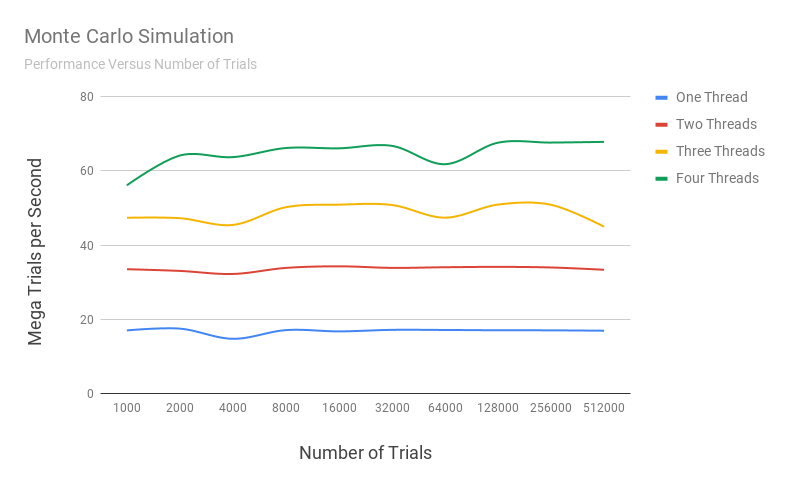
\includegraphics[width=\linewidth]{versusTrials.png}
      There is a dip for an input size of 64000,
      which probably reflects a slight dip in
      server load since these program executions
      were executed serially through a shell 
      script. There's an interesting dip in
      performance for the three threaded execution
      for large input sizes. 

    
    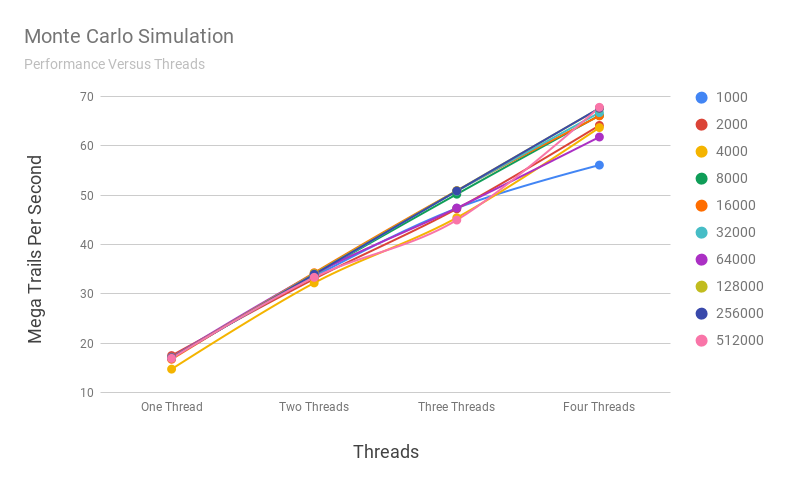
\includegraphics[width=\linewidth]{versusThreads.png}
    This graph illustrates that the performance 
    generally increases as the number of threads
    increases. Interestingly, the the blue line
    that represents an input size of 1000 seems
    to increase at a slower rate for the four
    threaded execution, which might be explained
    by the fact that smaller input sizes are more
    greatly affected by the overhead involved
    in delegating work among threads. Or it could
    be a fluke. 

  \item \textbf{Parallel Fraction} 
  
    My estimate for the parallel fraction is \textbf{1}. 
    I used the results from executing the code with four
    threads and with 512,000 number of trials to estimate
    the parallel fraction. If I choose instead the results from 
    two threads or three threads, the parallel fraction changes to
    0.98 or 0.93 respectively, so the estimate should be understood
    to have some error $<$ 0.1.

    Let $S_1$ and $S_4$ be the speeds
    of the program executed with one thread and four threads
    respectively. From my results, $S_1 = 16.96$ and $S_4 = 67.84$,
    so the speedup is $\frac{67.84}{16.96} = \mathbf{4}.$

    From Amdahl's law, we can solve for
    the parallel fraction, $P_f$:

    \begin{align*}
      S &= \frac{1}{\frac{F_p}{n} + (1 - F_p)}\\
      \frac{F_p}{n} + (1 - F_p) &= \frac{1}{S}\\
      \frac{F_p}{n} -F_p &= \frac{1}{S} - 1\\
      F_p(\frac{1}{n} -1) &= \frac{1}{S} - 1\\
      F_p &= \frac{\frac{1}{S} - 1}{\frac{1}{n} -1}\\
      F_p &= \frac{n(\frac{1}{S} - 1)}{1 - n}\\
      F_p &= \frac{n}{1-n}(\frac{1}{S} - 1)\\
      F_p &= \frac{n}{n - 1}(1 - \frac{1}{S})
    \end{align*}

    Subsituting 4 for n and 4 for S:

    \begin{align*}
      F_p &= \frac{4}{4 - 1}(1 - \frac{1}{4})\\
      F_p &= \mathbf{1}
    \end{align*}

\end{enumerate}
\end{document}
